\chapter{Testy}

\section{Testy integracyjne}

Testy integracyjne mają na celu sprawdzenie, czy interfejsy pomiędzy komponentami współdziałają ze sobą poprawnie\cite{mielnikIntegrationTests}. Do przeprowadzenia testów została użyta biblioteka "pytest", która pozwala na szybkie i proste uruchomienie testów. Do wykonywania zapytań HTTP została wykorzystana biblioteka "requests". Testy miały na celu sprawdzenie, czy status zwrócony przez wykonane żądanie pokrywa się z oczekiwanym rezultatem.\\
Przetestowane zostały poniższe funkcjonalności systemu:

\begin{itemize}
    \item Utworzenie fiszki
    \item Zwrócenie danych fiszki na podstawie id
    \item Aktualizacja danych fiszki
    \item Usunięcie fiszki
    \item Otrzymanie odpowiedzi od chatu GPT
    \item Tworzenie talii
    \item Zwrócenie danych talii na podstawie id
    \item Zwrócenie danych wszystkich talii należących do użytkownika
    \item Aktualizacja danych talii
    \item Usunięcie talii
    \item Zwrócenie rankingu talii
    \item Utworzenie konta użytkownika
    \item Logowanie do systemu
    \item Zwrócenie danych użytkownika
\end{itemize}

\begin{figure}[H]
    \centering
    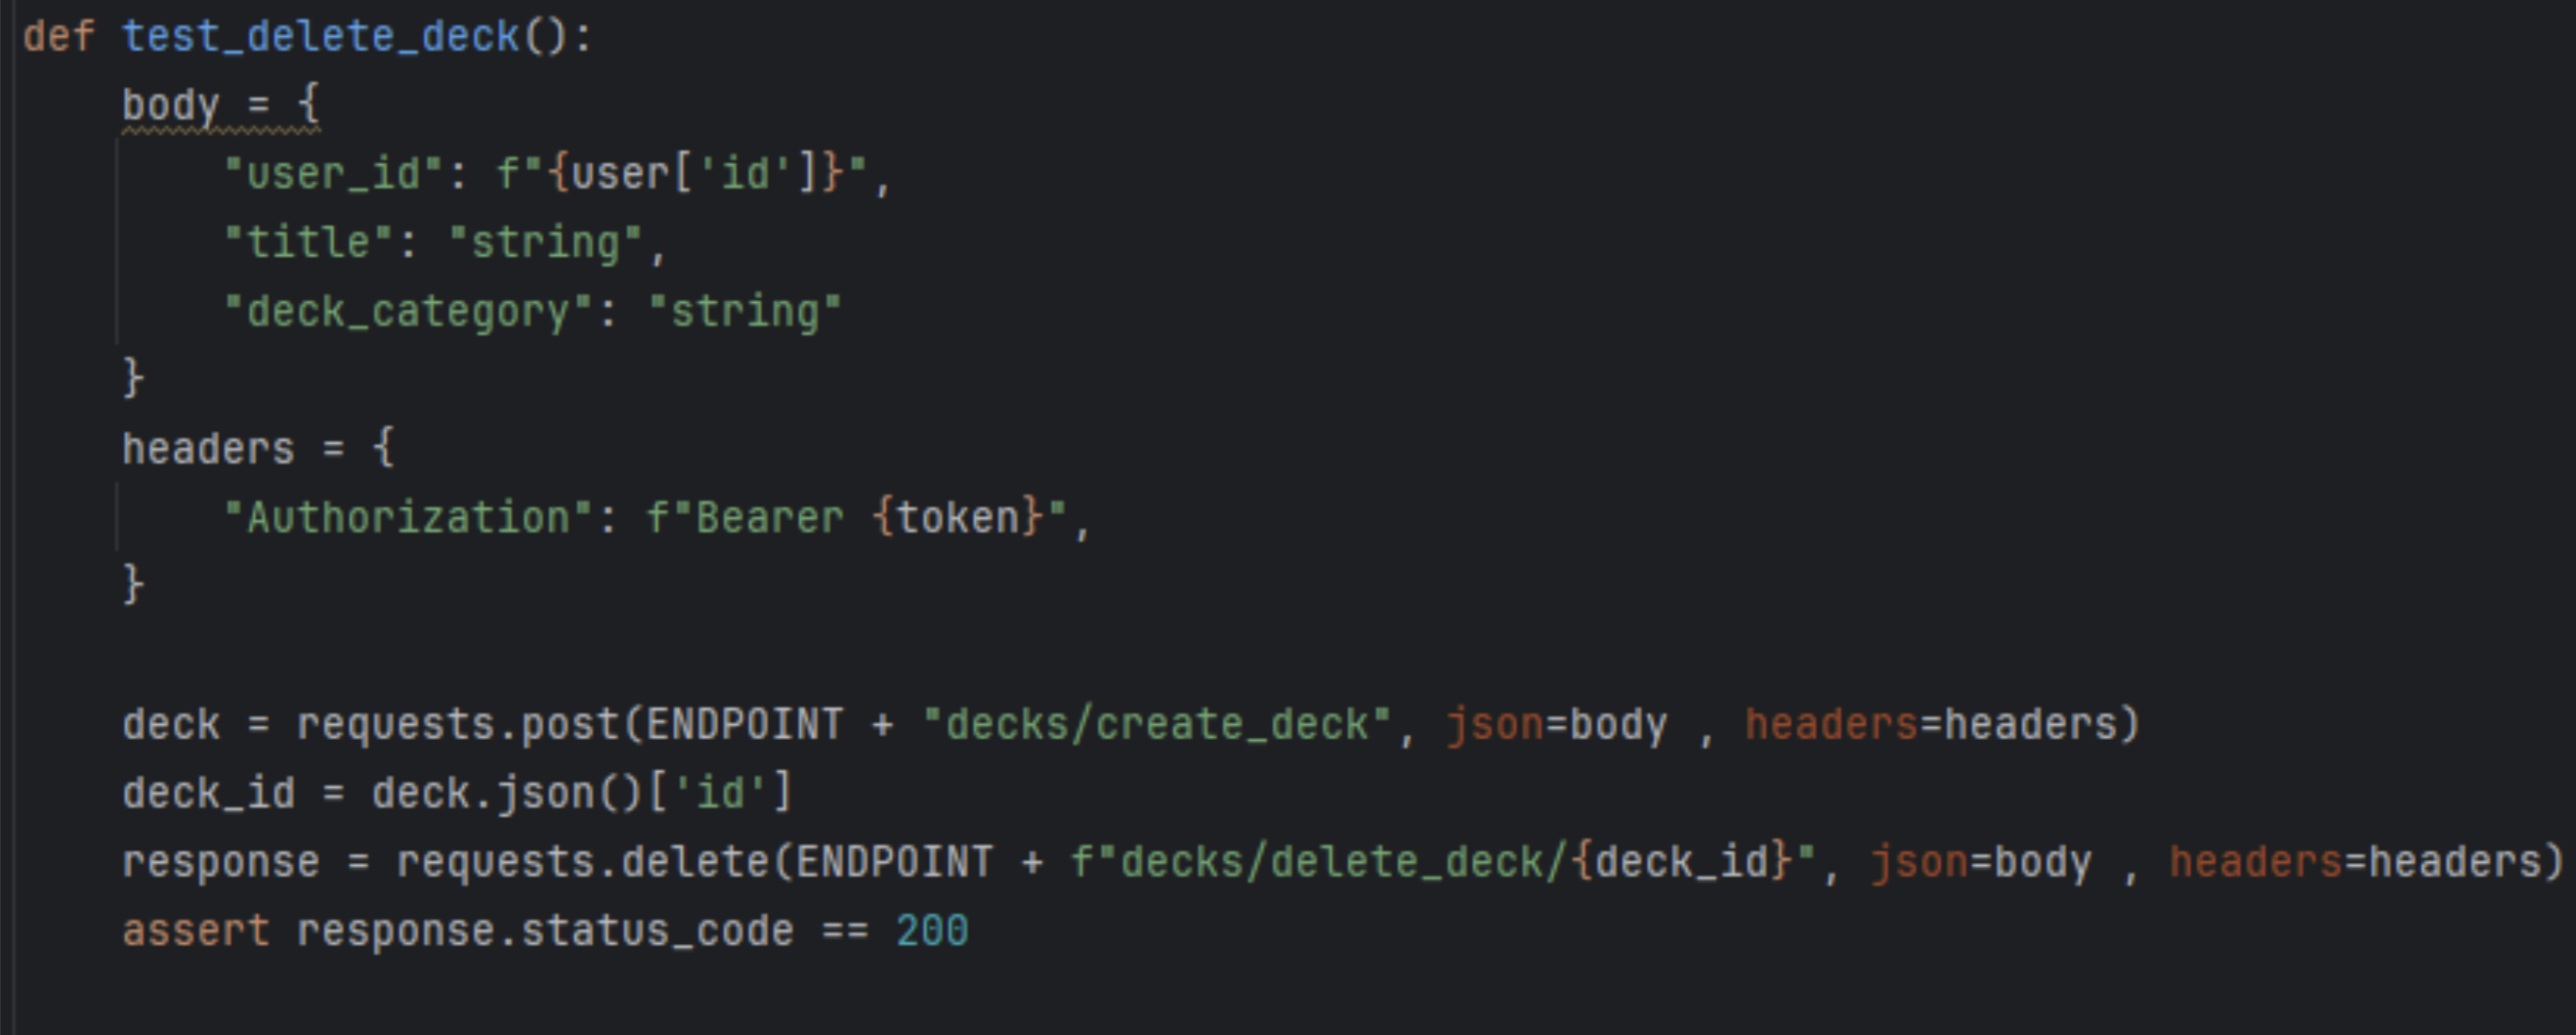
\includegraphics[width=1\textwidth]{chapters/chapter_9/testy1}
    \caption{Test sprawdzający działanie endpointu do usuwania talii użytkownika.}
    \label{img:testy}
\end{figure}

\section{Testy akceptacyjne}

Testy akceptacyjne pozwalają ocenić gotowość systemu do wdrożenia. Głównym ich założeniem jest sprawdzenie, czy system nadaje się do użytkowania. Zazwyczaj do testów akceptacyjnych wykorzystywana jest grupa użytkowników.\cite{acceptanceTesting} Do przeprowadzenia testów zostały sporządzone scenariusze testowe.


TBC